\documentclass{article}

\usepackage[hyphens]{url}
\usepackage{fontspec}
\usepackage{graphicx}

\graphicspath{ {./images/} }

\defaultfontfeatures{Mapping=tex-text,Scale=1.00}
\setmainfont{Inter Light}
\setmonofont{Liberation Mono}
% \usepackage[sfdefault,light]{inter} % this needs tex live
% \usepackage[T1]{fontenc}
\linespread{1.50}
\sloppy

\begin{document}
\title{The Craft of Code: Practice and Knowledge in the Production of Software}
\author{Pierre Depaz}
\date{January 2021}
\maketitle

\section{Introduction}

Software development as a practice has been developing for the past sixty years, emerging as a corollary from the field of computer science. In the 21st century, the importance of code in everyday lives has been highlighted from general-audience journalism\cite{ford_what_2015} to government initiatives\cite{wilson_hour_2015}. However, the distinction between programming and computer science is a blurry one. While a computer science degree does provides the appropriate formation for a programmer, successful programmers do not necessarily need a computer science background in order to be competent at their jobs. Indeed, while programming has historically emerged as an occupation which responded to the \textit{ad hoc} requirements of computing as a developing field\cite{chun_software_2005}, developing further into a codified and identified practice\cite{dijkstra_chapter_1972}, programming has nonetheless often been approached in media- and software- studies with a focus on the phenomenon of computation\cite{berry_philosophy_2011}, on the literary\cite{hayles_my_2010}, or on the social\cite{mackenzie_cutting_2006}, amongst others, rather than on the practice of programming as part of a historical tradition.

Starting from this observation, this article proposes to investigate a different tradition than that of the sciences to highlight the specificities of programming as a practice—the tradition of craftsmanship. Indeed, code isn't just code, but rather a myriad of socio-technical \textit{assemblages} composed of programming languages (e.g. Ruby, C, Julia, JavaScript), operating systems (e.g. Linux, BSD, OSX, Windows) and tools (e.g. IDEs, debuggers, compilers and processors). Those assemblages are in turn used within a cultural context made up of stories, sayings and texts, both from academic and folklore origins. This approach relies on a shift from a conceptual perspective of code, to one in which the word \textit{code} implies varieties of activities\cite{hayes_cultures_2017}, in which the variety of practices, self-identifications and narratives from programmers themselves is put at the forefront. The main distinction this article starts with is between computer scientist, as the theoretical approach to field of computation and the software developer, practical implementer, immersed in the practice of writing and reading code.

While links between craftsmanship and programming have existed as self-proclaimed ones by programmers themselves, as well as by academics and writers \cite{sennett_craftsman_2009,chandra_geek_2014}, they have not yet been elucidated under specific angles. Indeed, craftsmanship as such is an ever-fleeting phenomenon, a practice rather than a theory, in the vein of Michel De Certeau's \textit{tactics}, bottom-up actions designed and implemented by the users of a situation, product or technology as opposed to \textit{strategies}\cite{certeau_invention_1990}, in which ways of doing are prescribed in a top-down fashion. It is this practical approach that this article chooses, the informal manners and standards of working, in order to provide an additional, cultural studies perspective, to its media and software studies counterparts.

A comparative approach of a broad mode of economic and cultural activity (craftsmanship) with a narrower technical know-how (software development) asks us first to verify to what extent such an approach is even valid. How, then, is the designation by software developers of their own practice as craftsmanship relevant? Where is the comparison a productive one, and where does it show its limits? How can such comparison enrich both our understanding of code as a practice, as well as craftsmanship practices within the highly networked environment that has become the backdrop of the $21^{st}$ century? Particularly, how does it re-present processes of knowledge acquisition and aesthetic judgment?

The article proceeds in a comparative fashion, mobilizing texts about craftsmanship as well as sources from the field of programming, describing programmers' self-identification with craftsmanship. From those, I analyze how those references by programmers enter into a productive dialogue with our historical and cultural conception of craftsmanship. To do so, I approach these questions through three different, contiguous topics. First, the focus is set on the historical unfoldings of craftsmanship and software development, showing parallels. After inquiring into the modes of organization and the economical development of both craftsmanship and software development, this section focuses on a particular comparison: that of programming with building, and in particular its relationship with architecture. Second, we shift our focus from a broad view to the specific practices of knowledge acquisition and production. There, we highlight the similarities in terms of tacit and personal knowledge, as well as the means of education and information available both to traditional craftspeople and software developers. This, in turn allows us to discuss the differences of learning environments by taking into account the networks of environment that have developed exponentially with the Internet. Finally, the third section turns to aesthetic judgment of the crafted product. Building on discussions of beautiful craft and beautiful code, the focus here is on the standards which allow practicioners to ascribe beauty to a piece of software; particularly, this section discusses the materiality of code not in terms of bits, bytes and languages, but rather as a material that is worked with and worked through.

These incursions in the practices of software development via the lens of craftsmanship as a cultural practice concludes on the productive differences and similarities in terms of knowledge circulation and materialities when programming code; ultimately resulting in new understandings of both craftsmanship and software development as mutually influencing practices.

\section{Parallels}

This section starts by providing an overview of the various perspectives and realities on craftsmanship, starting from the Late Middle-Ages until the $20^{th}$ century. This allows us to highlight some initial important features of craftsmanship: social organization, the nature of work and the transmission of knowledge. Jumping to the history of software development, starting in the mid-$20^{th}$ century, it looks at the claims that programmers make about themselves in relation with the term and concept of craftsmanship. By examining formal and informal texts, we focus on the fact that software developers ground their practice in passion, know-how and myths. Finally, we inspect the place of architecture, both in historical craftsmanship and contemporary software development, in order to qualify further the relationship between design and implementation in those two fields.

\subsection{Craftsmanship through the ages}

Craftsmanship in our contemporary discourse seems most tied to a retrospective approach: it is often qualified as that which was \emph{before} manufacture, and the mechanical automation of production\cite{thompson_study_1934}. So while the practice of developing a skill in order to build something with a functional design has been considered at its apex of craftsmanship in Western late Middle-Ages, it should be noted here that non-Western craftsmanship are as equally rich and unique as their Western counterparts, for instance in China\cite{zhang_jingdezhens_2015} and Japan\cite{jordan_copying_2003}; however, these lie beyond the immediate scope of this article. Following Sennett, we will use his definition of craftsmanship as \emph{hand-held, tool-based, intrinsically-motivated work which produces functional artefacts, and in the process of which is held the possibility for unique mistakes}\cite{sennett_craftsman_2009}.

Late Middle-Ages craftsmanship stands out as such for a couple of reasons: their socio-economic organization, and their relationship to knowledge. First and foremost, craftspeople were indissociable from the guilds they belonged to\cite{black_guilds_1984}. As tightly-knit communities, they exhibited strong cohesion: vertically, between a master and their apprentices, and horizontally, between equal practicioners, enforcing a uniform quality control assurance and price management (Managerial Techniques by Wolek). This cohesion, in turn, has limited the amount of individual fame and glory that craftspeople could accumulate, as compared to fine-artists\cite{thompson_materials_1956}.

A key aspect of the craftsmanship of this time is the relationship that they maintained with explicit, formalized standards. While various crafts did include specific lexical fields to describe the details of their trade\cite{bassett_craftsman_2008}, usually compiled into glossaries, the standards for quality were less explicit. Cennino Cennini, in his \emph{Libro dell'arte}, one of the first codexes to map out technical know-how necessary to a painter in the early Renaissance, lays out both practical advice on specific painting techniques, but does not explicitly lay out how to make something \emph{good}\cite{cennini_craftsmans_2012}. Further work, at the eve of the Industrial Revolution, continued on this intent to formalize the practice of craftsmanship\cite{pannabecker_diderot_1994}. In this sense, quality work is rooted in implicit knowledge: a good craftsman knows a quality work when they see it\cite{sennett_craftsman_2009}. 

Another component of craftsmanship is its alleged incompatibility with manufacture\cite{ruskin_seven_1920,sturt_wheelwrights_1963}. However, studies have shown that the craftsmanship, rather than standing at the strict opposite of the industrial\cite{jones_reckoning_2016}, has been integrated into the process of modern industrialization. The practice of the craftsman, then, integrates into the design and operation of machines and industrial-scale organizations, informing ways of making in our contemporary world\cite{gordon_who_1988,mcgee_craftsmanship_1999}.

These characteristics of tight and rigid communities, implicit knowledge, and ambiguous separation with design, framing the foundation of a desire for good work are particularly highlighted in the field of the built environment, and later in the development of architecture. Before examining how such a field has a connection to software development, we take a look at programming's emergence as a field of craft.

\subsection{Software developers as craftsmen}

Computer programming as an activity came to be as an offshoot of computer science, perhaps best illustrated by the collaboration of Charles Babbage and Ada Lovelace on The Analytical Engine, the prototype of the modern computer. With Babbage acting as the overall designer, Lovelace was key in practically implementing some of the mathematical formulas which The Analytical Engine was built to solve. What we see here is a dyad of work, distinguished between design and conception on one side, and implementation and practice on the other side. These two approaches are echoed throughout the early days of programming (1950s-1970s), with programmers becoming distinct from computer scientists by their approach to the problem (they'd rather write code on a terminal than write algorithms on a piece of paper) and by their background (trained as scientists but more comfortable with tinkering)\cite{ensmenger_computer_2012}. In particular, the group of computer enthusiasts described as hackers developed organizational features similar to their historical counterparts: work was being done on distinct topics and fields in different geographic locations (Stanford, MIT, Bell Labs)\cite{raymond_cathedral_2001}, emphasis was put on engagement with tools (steaphenson), inquiring into peers' work\cite{levy_hackers_2010} and later formalized into bottom-up archives\footnote{The most famous of which is the Jargon File, later to be published as the The New Hacker's Dictionary: \url{http://www.catb.org/jargon/html/}}. Additionally, little accountability was required when it came to design explicitness. As examples, both the UNIX operating system and the TCP/IP protocol were originally realized without overarching supervision and without extensive ongoing documentation\cite{seibel_coders_2009,raymond_cathedral_2001}.

As computer science solidified as a distinct field in the 1960s\cite{tedre_development_2006}, there was a process of formalizing the hitherto \textit{ad hoc} techniques of programming computers. As a response to the myth of carefully hand-made code\footnote{See The Story of Mel, A Real Programmer, a folktale of early programmers: \url{https://www.cs.utah.edu/~elb/folklore/mel.html}} and unconstrained approaches to writing code came the structured programming approach, initally proposed by E. W. Djisktra\cite{dijkstra_chapter_1972}. With the operating system and the personal computer revolutions, access to tools became widespread, and transformed tightly communities into a global network of exchange, first via Usenet, then through the Web. Inquiries into the relationship of craftsmanship with programming started to take place in the mid-1970s from an educational perspective\cite{dijkstra_craftsman_1982}, from an organizational perspective\cite{brooks_mythical_1975} and an inter-personal perspective\cite{weinberg_psychology_1998}, and culminated with the publication of several trade books\cite{martin_clean_2008,hendrickson_software_2002}, explicitly connecting the craft of programming with previous craft activities, and emphasizing the need for intrinsic motivation and the aim of a job well-done\cite{hoover_apprenticeship_2009,goodliffe_code_2007}.

Comparisons of software development with craftsmanship are abundant, and relate then mostly to the relationship between unstructured practice and formalized theory; as such, it is used to self-categorize programmers as skilled makers rather than passive thinkers\footnote{See code monkey: \url{http://www.techopedia.com/definition/31469/code-monkey}}.

\subsection{The case of architecture}

The field of architecture helps us tie these two traditions together a little more explicitly. Architecture as a field and the architect as a role have been solidified during the Renaissance\cite{pevsner_term_1942}, consecrating a separation of abstract design and concrete work, in which the craftsman is relegated to the role of executioner, until the arrival of civil engineering and blueprints overwhelmingly formalized the discipline.

The classical architect, here, serves as the counterpart to the computer scientist, except in an inverse relation: the architect emerged from centuries of hands-on work, while the computer scientist (formerly known as mathematician) was first to a whole field of practicioners as programmers, followed by a need to regulate and structure those practices. Different sequences of events, perhaps, but nonetheless mirroring each other. On one side, construction work without an explicit architect, under the supervision of bishops and clerks, did indeed result in significant results (Notre Dame de Paris, Basilica of Sienna). On the other side, letting go of structured and restricted modes of working characterizing computer programming up to the 1980s resulted in a comparison described in the aptly-named \textit{The Cathedral and the Bazaar}. This essay described the Linux project, the open-source philosophy it propelled into the limelight, and how the quantity of self-motivated workers without rigid working structures (which is not to say without clear designs) can result in better work than if made by a few, select, highly-skilled individuals\cite{raymond_cathedral_2001,henningsen_joys_2020}.

What we see, then, is a similar result: individuals can cooperate on a long-term basis out of intrinsic motivation, and without clear, individual ownership of the result; a parallel seen in the similar concepts of \textit{collective craftsmanship} in the Middle-Ages and the \emph{egoless programming} of today\cite{brooks_mythical_1975}. The further sections will investigate how such a phenomena of building complex structures through horizontal networks is possible, from both epistemological and aesthetic perspectives.

\section{Knowledge acquisition and production}

\subsection{Bus factor and implicit knowledge}

The problem of knowledge in software development can be examplified by the "bus factor"\footnote{\url{https://en.wikipedia.org/w/index.php?title=Bus_factor}}. It describes the risk of crucial information being lost due to the disappearance or incapacity of one of the programmers of the project, and aims at the problem of \emph{essential complexity}\footnote{See the \textit{No Silver Bullet} essay in \emph{The Mythical Man-Month}, op.cit.}. Given the inherent complexity of programming as a task, along with the compulsive behaviours sometimes exhibited by programmers as a by-product of intrinsic motivation\cite{weizenbaum_computer_1976}, the gap between design and implementation---the domain of the craftsman---often relies on tacit knowledge\cite{collins_tacit_2010}.

Explicit knowledge, in programming as in most disciplines, is carried through books, academic programs and, more recently, web-based content that is either structured (e.g. MOOCs, Codeacademy, Khan Academy) or unstructured (e.g. blog posts, forums, IRC channels), but both seem to be insufficient to reach an expert level\cite{davies_models_1993}. As demonstrated by a popular comic, the road to good code is unclear, particularly when communicated in such a highly-formal language as diagramming. Given the fact that an individual can become a programmer through non-formal training---as opposed to, say, an engineer or a scientist---, the learning process must include implicit knowledge.

\begin{figure}
    \centering
    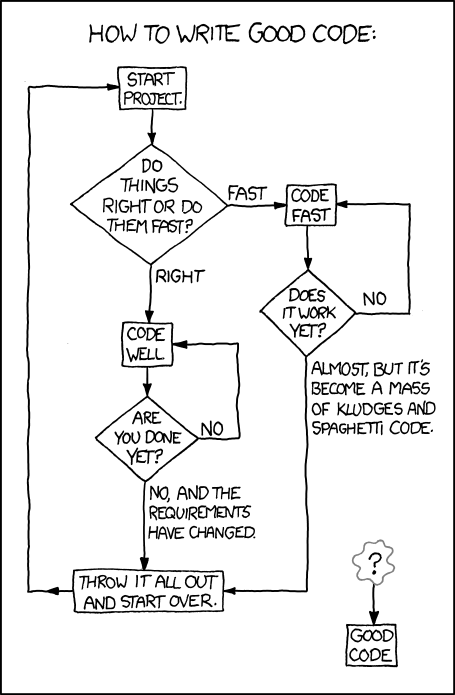
\includegraphics[scale=0.5]{good_code.png}
    \caption{Source: https://xkcd.com/844/}
\end{figure}


\subsection{Apprentices and masters}

The acquisition of such implicit knowledge in craftsmanship takes place in two different ways: the apprentice-master relationship, and the act of copying. First comes the apprentice-master relationship, in which a learner starts by  imitating the way of working of the master (Sennett), resulting in a \emph{teaching by showing}, where important aspects of the craft are being demonstrated to the apprentice by a more experienced practicioner, rather than formalized and learned \emph{a priori} of the practice. Sometimes, this relationship to a master is implemented explicitly through practices such as pair programming\cite{williams_pair_2003} or corporate mentorship programmings (IBM's Master programmer initiative). Other times, it is re-interpretated through fictional accounts designed to impart wisdom on the readers, and taking inspiration from Taoism and Zen\cite{james_tao_1987,raymond_new_1996}. From higher-level programming wisdom featuring leading programmers such as Marvin Minsky and Donald Knuth, this sort of informal teaching by showing has been implemented in various languages as a practical learning experience\footnote{See, for instance: \url{http://rubykoans.com/}}. Without the presence of an actual master, the programming apprentice nonetheless takes the program writer as their master to achieve each of the tasks assigned to them. The experience historically assigned to the master craftsman is delegated into the code itself, containing both the problem, the solution to the problem and hints to solve it, straddling the line between formal exercises and interactive practice.

Code's ability to be copied and executed on various machines provides a counterpoint to the argument of software as craftsmanship in terms of knowledge transmission. Traditionally, since craftsmanship has been understood as that which is done by hand, and since craftsmen were working with unique artefacts (i.e. no artefact can be perfectly copied), copying someone else's realization was physically inconceivable. The realm of software, on the opposite, relies heavily on the technical affordance of code to be duplicated, uploaded, downloaded and executed on multiple platforms through source code files\cite{manovich_language_2001}. The first immediate consequence of this is the ability for all to inspect and use source code, both on an institutional level (as guaranteed by projects such as GNU\footnote{See: \url{https:gnu.org}}), and on a vernacular level (as enabled by Web 2.0 platforms such as StackOverflow and GitHub). Even though the ability to perfectly copy anyone else's work became widely available to programmers, the difference between amateur and expert programmers lied in the extent to which they indeed blindly copy external code, or write their own, inspired by the external code\footnote{See the discussions on \url{https://softwareengineering.stackexchange.com/questions/36978}}.

Practices from Eastern craftsmanship further qualify these essentially different approaches to copying. \emph{Moxie}, a Chinese term for copying and practice, is a key concept to understand how an apprentice can equal his master through thougtful replication \cite{man_influence_2015}, an approach equally present in Japanese crafts histor\cite{jordan_copying_2003}. Here again, manually copying from established quality work to seize their elusive essence is an essential aspect to craftsmanship.

\subsection{The problem with copying}

If implicit knowledge can be acquired through a showing and copying of code, software development as a craft presents an additional dimension to this, a sort of \emph{piecemeal knowledge}. Best represented by Stack Overflow, a leading question and answer forum for programmers, on which code snippets are made available as part of the teaching by showing methodology, this piecemeal knowledge can both help programmers in solving issues as well as deter them in solving issues \textit{properly}\cite{treude_understanding_2017}. Code as such is freely and easily accessible as piecemeals, but often lacks the essential context.

So while programmers are to acquire implicit knowledge through a process of learning by doing (realizing koans, coding small projects, re-using copied code), we now need to assess how much of it happens through observing. Implied in the apprentice-master relationship is that what is observed should be of \textit{good quality}; one learns through ones own mistakes, and through ones presentation with exmaples of good work. Coming back to the relationship between architecture and software development, Christopher Alexander asks, in the preface of Richard P. Gabriel's \textit{Patterns of Software}\cite{gabriel_patterns_1998},

\begin{quote}
    \textit{For a programmer, what is a comparable goal? What is the Chartres of programming? What task is at a high enough level to inspire people writing programs, to reach for the stars?}
\end{quote}

If a craftsman learns their trade by comparing their work with work of a higher quality (either their master's, or publicly available works, assembled as a canon\cite{taylor_patterns_2001}), the programmer is faced with a different problem: a lot of examples, but a few good ones.  Copyright stands in the way of pedagogical copying. With software becoming protectable under copyright laws in the 1980s\cite{oman_computer_2018}, great works of programming craft became unacessible to programmers, despite the value they would bring in knowledge acquisition\cite{gabriel_mob_2001}. One of the most famous examples is \emph{Lions' Commentary on UNIX 6th Edition, with Source Code} by John Lions, an annotated edition of the UNIX source code, which was circulated illegaly in classrooms for twenty years before its official publication was authorized by the copyright owners\cite{lions_lions_1996}.

With implicit knowledge being a key component in both disciplines, its manifestation through the copying of source code in software development is hampered either by decontextualized, uploaded code snippets or by copyrighted protection on works, leading to a lack in an established canon of great works. Nonetheless, the other advice given to beginner programmers---practice\footnote{\url{https://quora.com/What-are-some-of-the-best-ways-to-learn-programming}}---hints at another aspect: direct engagement with code.

\section{Material aesthetics}

At the heart of knowledge transmission and acquisition stands the \emph{practice}, and inherent in the practice is the \emph{good practice}, the one leading to a beautiful result. This section investigates the aesthetics of code within the broader context of the aesthetics of craftsmanship, highlighting code's specificity as a material.

\subsection{The beauty of a thing well-made}

A traditional perspective is that of the motor skills, with dexterity, care and experience as essential features of a craftsman's ability to realize something beautiful\cite{osborne_aesthetic_1977}, along with self-assigned standards of quality\cite{pye_nature_2008,sennett_craftsman_2009}. These qualitative standards which, when pushed to their extreme, result in a craftsperson's \emph{style}, are to be gained through practice and experience, rather than by explicit measurements\cite{pye_nature_2008} \footnote{See Pye's account of craftsmanship, and his intent to make explicit the question of quality craftsmanship and \emph{"answer factually rather than with a series of emotive noises such as protagonists of craftsmanship have too often made instead of answering it."}}. Two things are concerned here: tools and materials\cite{pye_nature_2008}. A craftsperson should have a deep, implicit knowledge of both, what they use to manipulate (chisels, hammers, ovens, etc.) as well as what they manipulate (stone, wood, steel, etc).

This relationship to tools and materials is expected to have a relationship to \emph{the hand}, and at first seems to exclude the keyboard-based practice of programming. But even within a world in which automated machines have replaced hand-held tools, Osborne writes:

\begin{quote}
    \textit{In modern machine production judgement, experience, ingenuity, dexterity, artistry, skill are all concentrated in the programming before actual production starts.\cite{osborne_aesthetic_1977}}
\end{quote}

He opens here up a solution to the paradox of the hand-made and the computer-automated, as programming emerges from the latter as a new skill. This very rise of automation has been criticized for the rise of a Osborne's ``soulless society''\cite{osborne_aesthetic_1977}, and has triggered debates about authorship, creativity and humanity at the cross-roads between artificial intelligence and artistic practice\cite{mazzone_art_2019}. One avenue out of this debate is human-machine cooperation, first envisioned by Licklider and proposed throughout the development of Human-Computer Interaction\cite{licklider_man-computer_1960,grudin_tool_2016}. If machines, more and more driven by computing systems, have replaced traditional craftsmanship's skills and dexterity, this replacement can nonetheless suggest programming as a distinctly 21st-century craftsmanship, as well as other forms of cratsmanship-based work in an information economy.

\subsection{Code as material}

Beautiful code, code well-written, is indeed an integral part of software craftsmanship\cite{oram_beautiful_2007}. More than just function for itself, code among programmers can, and should be held to beauty standards\cite{pineiro_aesthetics_2003}. Such standards are another relationship with traditional craftsmanship---form following function.

A craftsman's material consciousness is recognized by the anthropomorphic qualities ascribed by the craftsman to the material\cite{sennett_craftsman_2009}. In the case of code, adjectives such as "clean", "elegant", "smelly" occur over and over in online discussions of programmers. Clean code, elegant code, are indicators not just of the awareness of code as a raw material that should be worked on, but also of the necessities for code to exist in a social world. As software craftsmen assemble in loose hierarchies to construct software, the aesthetic standard is \emph{the respect of others}\cite{abelson_structure_1979}.

Another unique feature of software craftsmanship is its blending between tools and material: code, indeed, is both. This is, for instance, represented at its extreme by languages like LISP, in which functions and data are treated in the same way\cite{mccarthy_lisp_1965}. In that sense, code is a material which can be almost seamlessly converted from information to information-\emph{processing}, and vice-versa. Disregarding for now the very real impact of computing on the environment\cite{kurp_green_2008}, code as a material is perhaps the only non-finite material that craftspeople can work with---along with words.

Code, then, is not just an overarching, theoretical concept which can only be reckoned with in the abstract, but also the very material foundation from which the reality of software craftsmanship evolves. An analysis of computing phenomena, from software studies to platform studies, should therefore take into account the close relationship to their material that software developers can have. As Fred Brooks put it,

\begin{quote}
    \textit{The programmer, like the poet, works only slightly removed from pure thought-stuff. He builds his castles in the air, from air, creating by exertion of the imagination. Few media of creation are so flexible, so easy to polish and rework, so readily capable of realizing grand conceptual structures.\cite{brooks_mythical_1975}}
\end{quote}

\subsection{The implications of beautiful code}

So while there are arguments for developing a more rigorous, engineering conception of software development\cite{ensmenger_computer_2012}, a crafts ethos based on a materiality of code holds some implications both for programmers and for society at large.

On the one side, since craftsmanship aesthetic standard relies on the process and the immediate usage of the product, little attention might be given to the long-term consequences of such a product. When computing systems start to get entangled with complex domains such as culture\cite{seaver_captivating_2019} or education\cite{perrotta_programming_2020}, programmers play a significant role in the development of these systems\cite{levy_programmation_1992}, and their intrinsic motivation to work with code for its own sake without a broader perspective might lead to undesired outcomes---a situation in which the function of the product is no longer beautiful.

On the other side, this engagement with code-as-material opens up possibilities for the acknowledgement of a different moral standard. As Pye puts it,

\begin{quote}
    \textit{[...] but still the quality of the result is clear evidence of competence and assurance, and it is an ingredient of civilization to be continually faced with that evidence, even if it is taken for granted and unremarked.\cite{pye_nature_2008}}
\end{quote}

If most commentators on the history of craftsmanship, following Ruskin, lament the disappearance of a better, long-gone way of doing things, before computers came to automate everything, locating software as a contemporary iteration of the age-old ethos of craftsmanship opens-up the possibility for a more conscious, careful and diligent way of building the future.

\section{Conclusion}

After qualifying a relationship to craftsmanship that has been claimed by software developers since the mid-1980s by a parallel with craftsman building and programming work, we've shown how these practicioners evolve in a somewhat different environment. First, their relation to knowledge and the need to acquire and transfer tacit knowledge has been limited by both the disappearance of strict master-apprentice relationships, and the removal from the public domain of some of software development's greatest achievements. Second, their relationship to code, as both materials and tools, while holding intrinsically the possibility for better, and more moral work, re-states the importance of code as a product which can be studied, learned and perfected.

\bibliographystyle{unsrt}
\bibliography{article}

\end{document}